\documentclass[10pt]{beamer}

\usetheme{metropolis}
\usepackage{appendixnumberbeamer}

\usepackage{booktabs}
\usepackage[scale=2]{ccicons}

\usepackage{pgfplots}
\usepgfplotslibrary{dateplot}

\usepackage{xspace}
\newcommand{\themename}{\textbf{\textsc{metropolis}}\xspace}

\title{Deep Learning Project: Synthesis}
\subtitle{Generating images by training Generative Adversarial Networks (GANs)}
\date{\today}
\author{Johannes Loevenich}
\institute{University of Bonn}
% \titlegraphic{\hfill\includegraphics[height=1.5cm]{logo.pdf}}

\begin{document}

\maketitle

\begin{frame}{Table of contents}
  \setbeamertemplate{section in toc}[sections numbered]
  \tableofcontents[hideallsubsections]
\end{frame}

\section{Motivation}

{
\metroset{titleformat frame=allcaps}
\begin{frame}{Generative Adversarial Networks}
      \begin{block}{Motivation}
	\begin{itemize}[<+- | alert@+>]
    \item Understanding Generative Adversarial models especially DCGAN's.
    \item Can we measure the quality of the \textbf{discriminator} by removing the real/fake classifier and feeding the convolutional features into a new classifier? This would show that the model learned general, useful features.
    \item Is it possible to show that there are dedicated parts of the \textbf{generator} that control properties of its output? In other words, do we reach some vector arithmetics on the input vector noise.
  \end{itemize}
    \end{block}
\end{frame}
}

\section{Training experiences}

{
\metroset{titleformat frame=allcaps}
\begin{frame}{Generative Adversarial Networks}
      \begin{block}{Motivation}
	\begin{itemize}[<+- | alert@+>]
    \item Training a DCGAN is some kind of an art.
    \item While training the DCGAN on IMAGENET-1K the \textbf{discriminator} always got too strong. 
    \item We had to interrupt training periodically and then just trained the \textbf{generator} for a few epochs. 
    \item With our GPU time it was not possible to reach nearly a good classification accuracy as they did in the papers.
    \item Training on celebA worked well and we got some nice results for the vector arithmetics. 
  \end{itemize}
    \end{block}
\end{frame}
}

\section{Theory}

{
\metroset{titleformat frame=allcaps}
\begin{frame}{Generative Adversarial Networks}
      \begin{block}{What is a GAN?}
	\begin{itemize}[<+- | alert@+>]
    \item GANs are a framework for teaching a DL model to capture the training data’s distribution so we can generate new data from that same distribution.
    \item They are made of two distinct models, a \textbf{generator} and a \textbf{discriminator}.
    \item The job of the \textbf{generator} is to spawn ‘fake’ images that look like the training images.
    \item The job of the \textbf{discriminator} is to look at an image and output whether or not it is a real training image or a fake image from the generator.
  \end{itemize}
    \end{block}
\end{frame}
}

{
\metroset{titleformat frame=allcaps}
\begin{frame}{Generative Adversarial Networks}
      \begin{block}{Discriminator Notation}
	\begin{itemize}[<+- | alert@+>]
    \item Let x be data representing an image. $D(x)$ is the discriminator network which outputs the (scalar) probability that $x$ came from training data rather than the generator. 
    \item Here, since we are dealing with images the input to $D(x)$ is an image of HWC size $3x64x64$. \item Intuitively, $D(x)$ should be HIGH when $x$ comes from training data and LOW when $x$ comes from the generator.
  \end{itemize}
    \end{block}
\end{frame}
}

{
\metroset{titleformat frame=allcaps}
\begin{frame}{Generative Adversarial Networks}
      \begin{block}{Generator Notation}
	\begin{itemize}[<+- | alert@+>]
    \item For the generator’s notation, let $z$ be a latent space vector sampled from a standard normal distribution.
    \item $G(z)$ represents the generator function which maps the latent vector z to data-space. 
    \item The goal of $G$ is to estimate the distribution that the training data comes from $p_{data}$ so it can generate fake samples from that estimated distribution $p_g$.
    \item So, $D(G(z))$ is the probability (scalar) that the output of the generator G is a real image.
  \end{itemize}
    \end{block}
\end{frame}
}
{
\metroset{titleformat frame=allcaps}
\begin{frame}{Generative Adversarial Networks}
      \begin{block}{Training by playing a MinMax game}
	\begin{itemize}[<+- | alert@+>]
    \item As described in Goodfellow’s paper, $D$ and $G$ play a \textbf{MinMax game} in which $D$ tries to maximize the probability it correctly classifies reals and fakes $(\log D(x))$, and $G$ tries to minimize the probability that $D$ will predict its outputs are fake $(\log (1 - D(G(x)) ))$.
    \item The GAN \textbf{loss function} is:
    $$\min_G \max_D V(D,G) = \mathbb{E}_{x \sim p_{data}(x)}[\log D(x)]+\mathbb{E}_{z \sim p_z(z)}[\log(1−D(G(x)))]$$
    \item In theory, the solution to this \textbf{MinMax} game is where $p_g$ = $p_{data}$
    and the discriminator guesses randomly if the inputs are real or fake. 
  \end{itemize}
    \end{block}
\end{frame}
}

{
\metroset{titleformat frame=allcaps}
\begin{frame}{Generative Adversarial Networks}
      \begin{block}{What is a DCGAN?}
	\begin{itemize}[<+- | alert@+>]
    \item A \textbf{DCGAN} is a direct extension of the \textbf{GAN} described above, except that it explicitly uses convolutional and convolutional-transpose layers in the discriminator and generator, respectively.
    \item The \textbf{discriminator} is made up of strided convolution layers, batch norm layers, and LeakyReLU activations. 
    \item The input is a $3x64x64$ input image and the output is a scalar probability that the input is from the real data distribution. 
    \item The \textbf{generator} is comprised of convolutional-transpose layers, batch norm layers, and ReLU activations.
    \item The input is a latent vector, $z$, that is drawn from a standard normal distribution and the output is a $3x64x64$ RGB image.
  \end{itemize}
    \end{block}
\end{frame}
}

{
\metroset{titleformat frame=allcaps}
\begin{frame}{Structure of the DCGAN network}
\begin{figure}[htbp] 
  \centering
     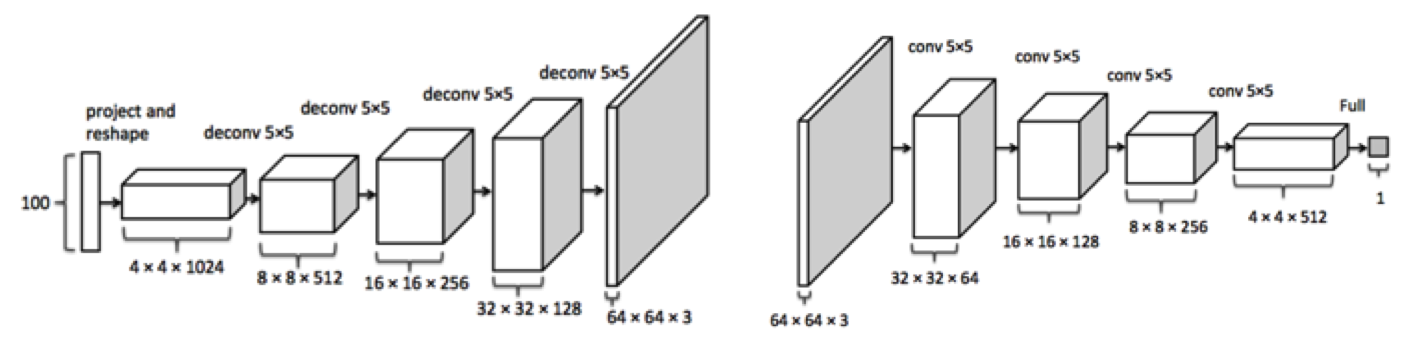
\includegraphics[width=1.0\textwidth]{pic/structure_dcgan.png}
  \caption{DCGAN network}
  \label{fig:Bild1}
\end{figure}
\end{frame}
}

\section{Experiment 1: Classification of Food-101}


{
\metroset{titleformat frame=allcaps}
\begin{frame}{Classification on Food-101}
      \begin{block}{The Data:}
	\begin{itemize}
    \item IMAGENET-1K: pictures of 1000 different objects
    \item food-101: 101.000 images in 101 different food categories
  \end{itemize}
    \end{block}
        \begin{block}{The Experiment:}
	\begin{itemize}
	\item Train a DCGAN on the IMAGENET-1K dataset. Use the \textbf{discriminator} as feature extractor for food-101. 
	\item Use the output of all the convolutional layers of the \textbf{discriminator} as feature extractor and train a linear SVM on food-101.
  \end{itemize}
    \end{block}
\end{frame}
}
{
\metroset{titleformat frame=allcaps}
\begin{frame}{Results Classification on Food-101}
      \begin{block}{Overall accuracy}
	\begin{itemize}[<+- | alert@+>]
    \item We tested the \textbf{discriminator} as feature extractor on the whole food-101 dataset (101.000 pictures in 101 categories) and on 10 random categories.
    \item To measure our classification results we used the models overall \textbf{accurracy} and \textbf{precision} and \textbf{recall} on each of datasets classes. 
    \item While \textbf{recall} expresses the ability to find all relevant instances in a dataset, \textbf{precision} expresses the proportion of the data points our model says was relevant actually were relevant.
    $$ recall = \frac{tp}{tp + fn} $$
    $$ precision = \frac{tp}{tp + fp}$$
  \end{itemize}
    \end{block}
\end{frame}
}

{
\metroset{titleformat frame=allcaps}
\begin{frame}{Results Classification on Food-101}
\begin{figure}[htbp] 
  \centering
     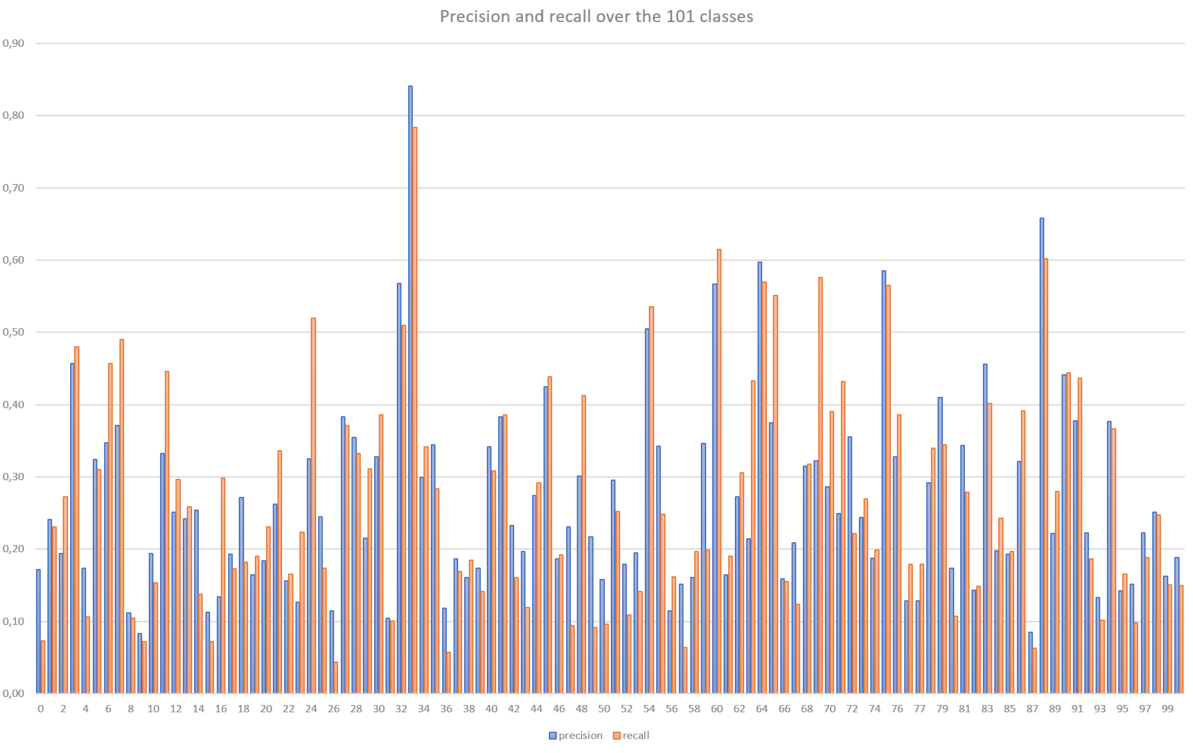
\includegraphics[width=1.0\textwidth]{pic/precision_recall_full.PNG}
  \caption{precision vs. recall over all 101 food categories }
  \label{fig:Bild1}
\end{figure}
\end{frame}
}

{
\metroset{titleformat frame=allcaps}
\begin{frame}{Results Classification on Food-101}
\begin{figure}[htbp] 
  \centering
     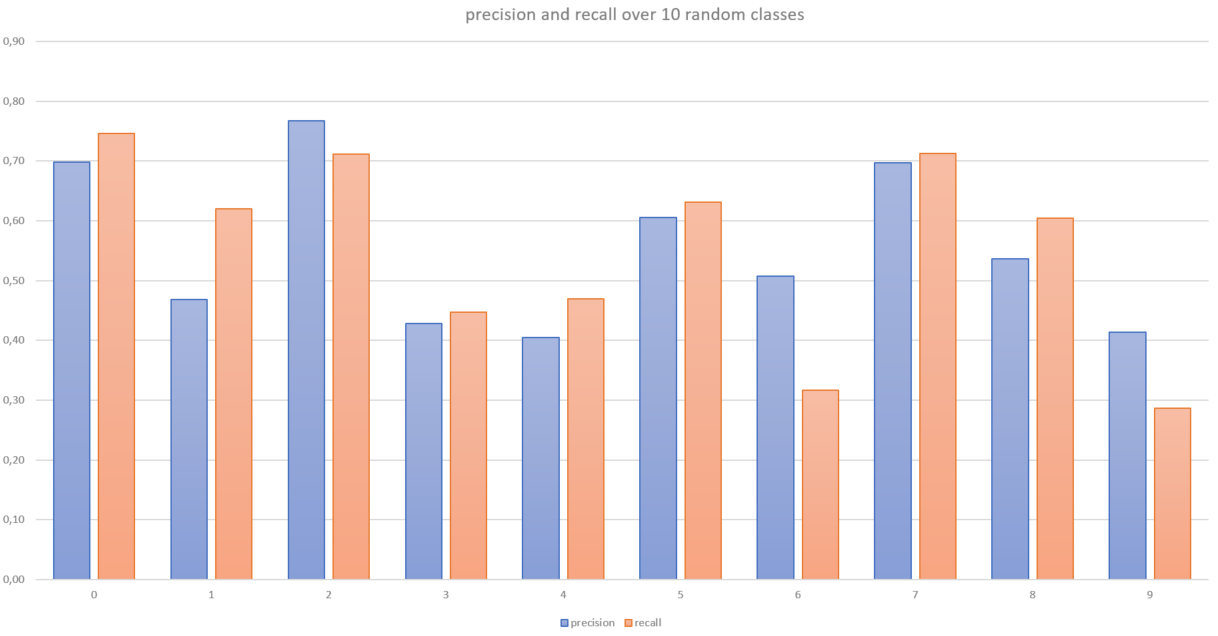
\includegraphics[width=1.0\textwidth]{pic/precision_recall_10_classes.PNG}
  \caption{precision vs. recall over 10 random food categories }
  \label{fig:Bild1}
\end{figure}
\end{frame}
}

\section{Experiment 2: LSUN conference-room}

{
\metroset{titleformat frame=allcaps}
\begin{frame}{LSUN conference-room}
      \begin{block}{The Data:}
	\begin{itemize}
    \item LSUN conference room: 229.069 images of conference-rooms
  \end{itemize}
    \end{block}
        \begin{block}{The Experiment:}
	\begin{itemize}
	\item Train a \textbf{Generator} on the LSUN conference-room dataset. 
  \end{itemize}
    \end{block}
\end{frame}
}

{
\metroset{titleformat frame=allcaps}
\begin{frame}{LSUN conference-room}
      \begin{block}{Generator and Discriminator losses}
	\begin{itemize}[<+- | alert@+>]
    \item \textbf{$Loss_D$} : \textbf{discriminator loss} calculated as the sum of losses for the all real and all fake batches $ \log(D(x))+\log(D(G(z)))$.
    \item \textbf{$Loss_G$}: \textbf{generator loss} calculated as $\log(D(G(z)))$
  \end{itemize}
    \end{block}   
\begin{figure}[htbp] 
  \centering
     \includegraphics[width=1.0\textwidth]{pic/lsun_losses.png}
  \caption{Generator and discriminator loss during training }
  \label{fig:Bild1}
\end{figure} 
\end{frame}
}

{
\metroset{titleformat frame=allcaps}
\begin{frame}{LSUN conference-room Real vs. Fake}
\begin{figure}[htbp] 
  \centering
     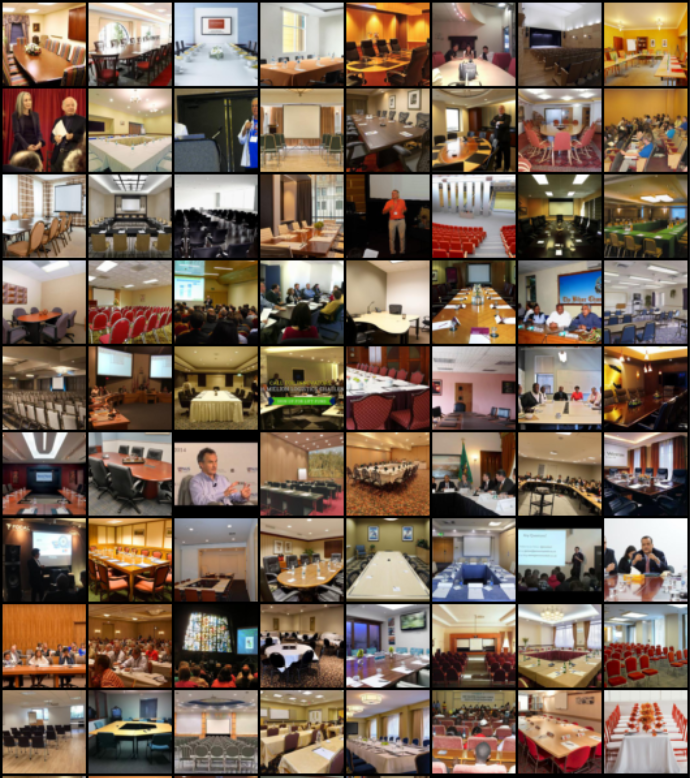
\includegraphics[width=0.65\textwidth,height=0.65\textwidth]{pic/lsun_real.PNG}
  \caption{Real samples from the LSUN conference-room dataset }
  \label{fig:Bild1}
\end{figure}
\end{frame}
}

{
\metroset{titleformat frame=allcaps}
\begin{frame}{LSUN conference-room Real vs. Fake}
\begin{figure}[htbp] 
  \centering
     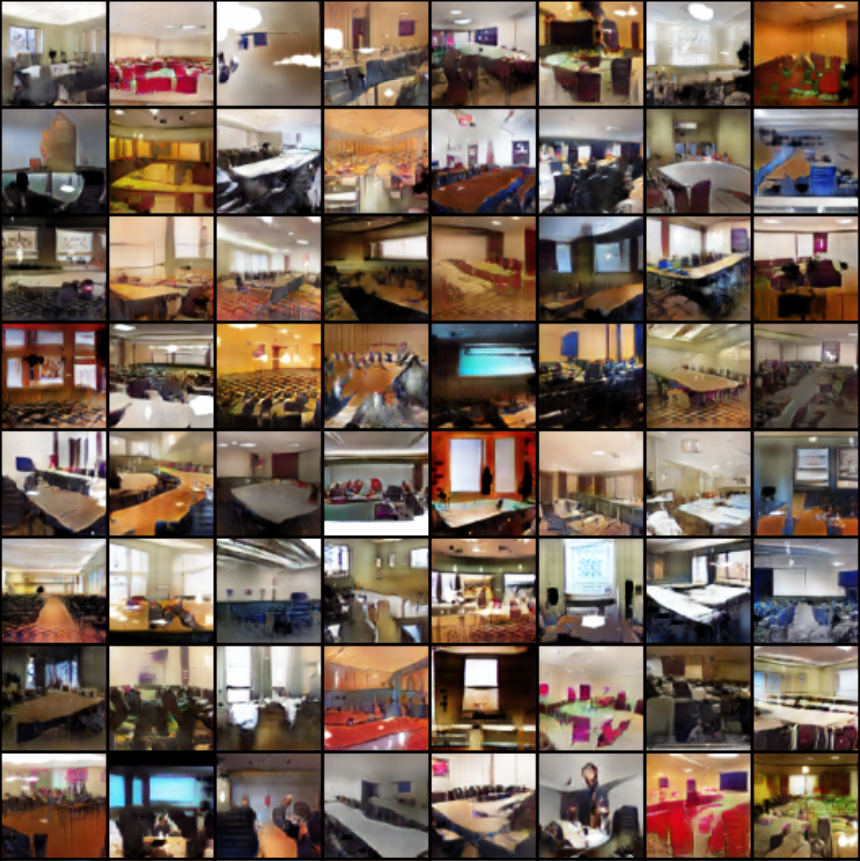
\includegraphics[width=0.65\textwidth,height=0.65\textwidth]{pic/lsun_fake.PNG}
  \caption{Fake samples after 25 epochs }
  \label{fig:Bild1}
\end{figure}
\end{frame}
}

\section{Experiment 3: Vector arithmetics for celebA}

{
\metroset{titleformat frame=allcaps}
\begin{frame}{Vector arithmetics for celebA}
      \begin{block}{The Data:}
	\begin{itemize}
    \item celebA faces dataset: 10.177 number of identities
    , 202.599 number of face images
  \end{itemize}
    \end{block}
        \begin{block}{The Experiment:}
	\begin{itemize}
	\item Train a \textbf{DCGAN} on the celebA faces dataset. Take two sets of 3 normal distributed sample vectors $A$ and $B$. Calculate both subsets means ($mean(A)$ and $mean(B)$). Then return the \textbf{generator's} output of $mean(a) + mean(B)$.
  \end{itemize}
    \end{block}
\end{frame}
}

{
\metroset{titleformat frame=allcaps}
\begin{frame}{Results Vector arithmetics for celebA}
\begin{figure}[htbp] 
  \centering
     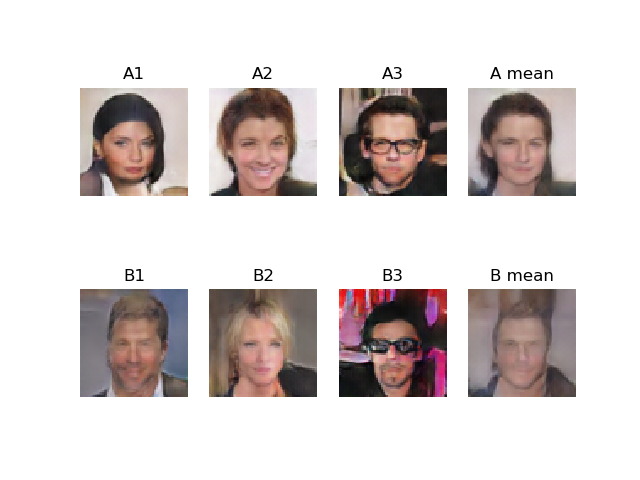
\includegraphics[width=0.65\textwidth,height=0.65\textwidth]{pic/experiment_2.png}
  \caption{Means }
  \label{fig:Bild1}
\end{figure}
\end{frame}
}

{
\metroset{titleformat frame=allcaps}
\begin{frame}{Results Vector arithmetics for celebA}
\begin{figure}[htbp] 
  \centering
     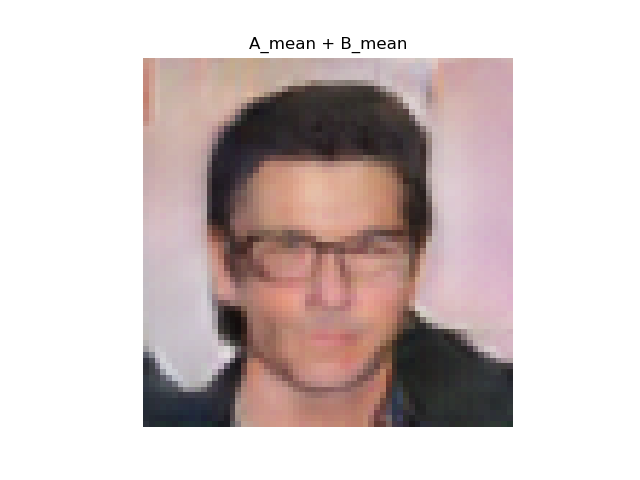
\includegraphics[width=0.65\textwidth,height=0.65\textwidth]{pic/A_B_experiment_2.png}
  \caption{Sum of the means }
  \label{fig:Bild1}
\end{figure}
\end{frame}
}


\begin{frame}[standout]
  Questions?
\end{frame}\end{document}
